% chap3.tex (Definitions and Theorem)

\chapter{Sensor Data Provenance Collection Framework for the IoT}

In this chapter, we introduce a novel approach for how provenance is collected and modeled along the IoT architectural stack. We also propose a design and  implementation of such an IoT provenance collection framework. This section defines a model for relaying provenance in IoT systems which is built on top of PROV-DM. 

\section{IoT Provenance-Collection Framework }
%This section discusses the data model in which we represent sensor and actuator reading of provenance data collected from IoT devices . It also talks about the relationship between IoT provenance Collection and PROV\-DM; How data is process and disseminated across the IoT architecture.
%
%\textcolor{red}{TODO: Talks about how we use PROV\-DM and what kinds of provenance we are looking to store}

A provenance model is used to represent causal dependency between objects and it is usually represented as a Directed Acyclic Graph (DAG). This representation facilitates visualization of provenance relationships and offers a unified format for representing provenance data. We chose PROV-DM as the model to represent provenance for our implementation because it allows for the proper representation of all of the relationships in which we envision for IoT devices. 
From the IoT architecture as illustrated in Figure \ref{architecture}, data is disseminated from sensors and actuators across layers of the IoT architectural stack. The provenance data produced from various sensors and actuators are collectively aggregated at the gateway or the cloud layers. We translate provenance data to PROV-DM format at any layer of the IoT stack. This allows processing of provenance at all layers even in the case of a network failure. 
 Figure \ref{aggregation} illustrates the provenance data aggregation across the layers of the stack. Data is collected from sensors and actuators aggregated, and passed along the hierarchy. 


\begin{figure}[h!]
\begin{center}

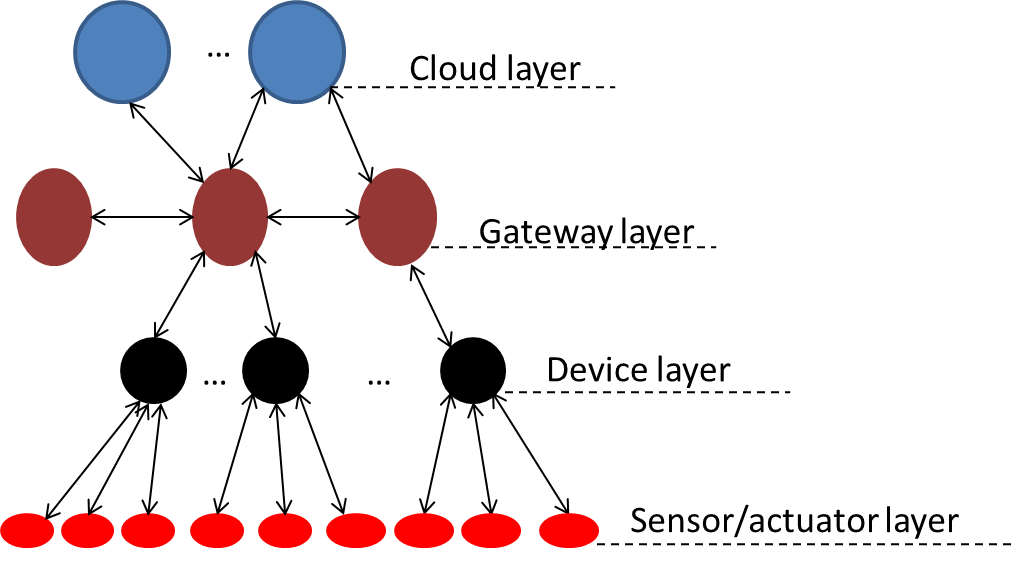
\includegraphics[width=3.0in]{iot_aggregation.PNG}    
\end{center}
\caption{IoT provenance-collection data aggregation showing how provenance data is aggregated across the various layers of the IoT architecture}
\label{aggregation}
\end{figure}


Using the scenario of a smart home as illustrated in chapter 2, a detailed example of how our provenance collection framework can be applied as follows:

\begin{itemize}

\item Provenance data is collected from sensor and actuator readings of devices contained in the smart home (e.g thermostat, refrigerator, and smart doors). The provenance data is collected as specified in a policy document. 

\item Provenance data from multiple sensor and actuator readings collected from each device are aggregated and passed along to the gateway, which transmits it to the cloud for long-term storage and use in data analytics. Each layer in the provenance IoT architecture is independent of other layers and maintains provenance information that can be mapped using the PROV-DM format which allows for the representation of dependencies between sensor-actuator readings contained in the device. This allows for analysis at each layer independently. 

\end{itemize}





\subsection{Provenance-Collection Model Definition}

 Since PROV-DM provides a generic model for representing provenance information, we define a more specific model for representing provenance data in IoT devices based on  PROV-DM. In the context of IoT provenance, we define entity, process and agent as follows:

\begin{itemize}

\item Agent: An agent is any data object that is responsible for the actions of an activity. An agent could also be an entity or an activity. Examples of agents in an IoT architecture are sensors, actuators, user roles (e.g admin). A unique identifier is given to each agents contained in an IoT framework.

\item Entity:  An entity can be defined as a data object that contains information which can be modifiable. An example entities are device files, processes, device memory contents and network packets. An Entity is identified by an id and can include additional attributes such as location and time.

\item Activity: An activity is an action that an agent makes on an entity. Examples of activities are basic file access operations such as read, write, delete, update, memory access such as load and store, and network activity such as send and receive. 


\end{itemize}


To better explain the provenance-collection model, a use case is illustrated in Figure \ref{prov_model}, which depicts a model for a smart home.



\begin{figure}[h]
\begin{center}

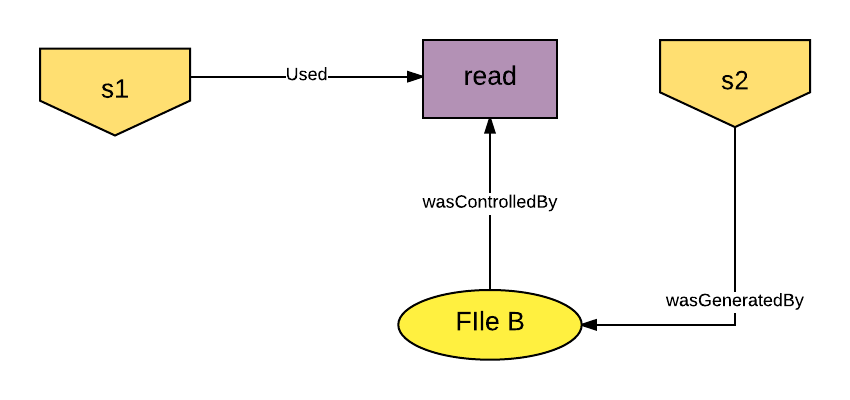
\includegraphics[width=4.0in]{prov_model_usecase.png}    
\end{center}
\caption{Provenance-model use case illustrating dependency relationship between two sensors, s1 and s2 }
\label{prov_model}
\end{figure}



Figure \ref{prov_model}  depicts a dependency relationship between two sensors, s1 and s2. s1 is a smart thermostat which regulates the temperature of the home and s2 is a sensor that detects the temperature of the environment. s1 checks the temperature of the environment in order to regulate the temperature of the house accordingly. s1 tries to access sensor temperature information from s2. According to the provenance data model  definition, s1 and s2 are agents. The activity performed on s2 by s1 is read. Sensor data from s2 is stored in File B which is  an entity that s1 tries to read sensor readings from s2. The relationship between components in the model is illustrated on the edges between types in the provenance model. We use the same relations contained in PROV-DM to represent relationships between types contained in the IoT framework.




\section{Provenance-Collection System}

In this section, we show how components of our system and describe how provenance trace is collected across the IoT framework. Figure \ref{architecture} displays the system architecture of our approach. Sensor and actuator readings in the form of input and output (I/O) events are recorded by the tracer component. This component intercepts system level I/O events and produces trace information represented in Common Trace Format (CTF). CTF encodes binary trace output information containing multiple streams of binary events such as I/O activity. Trace information is converted to provenance data in the PROV-DM IoT model and serialized to PROV-JSON. CTF conversion to PROV-DM will be achieved using babeltrace. This conversion can happen at any layer of the IoT stack. Babeltrace is a plugin framework which allows the conversion of CTF traces into other formats. Trace or provenance data is securely transmitted to a gateway and later transmitted and stored in a cloud backend. Our backend of choice is Neo4j, a graph database for efficient storage, query and visualization of provenance data.


\begin{figure}[b]
\begin{center}

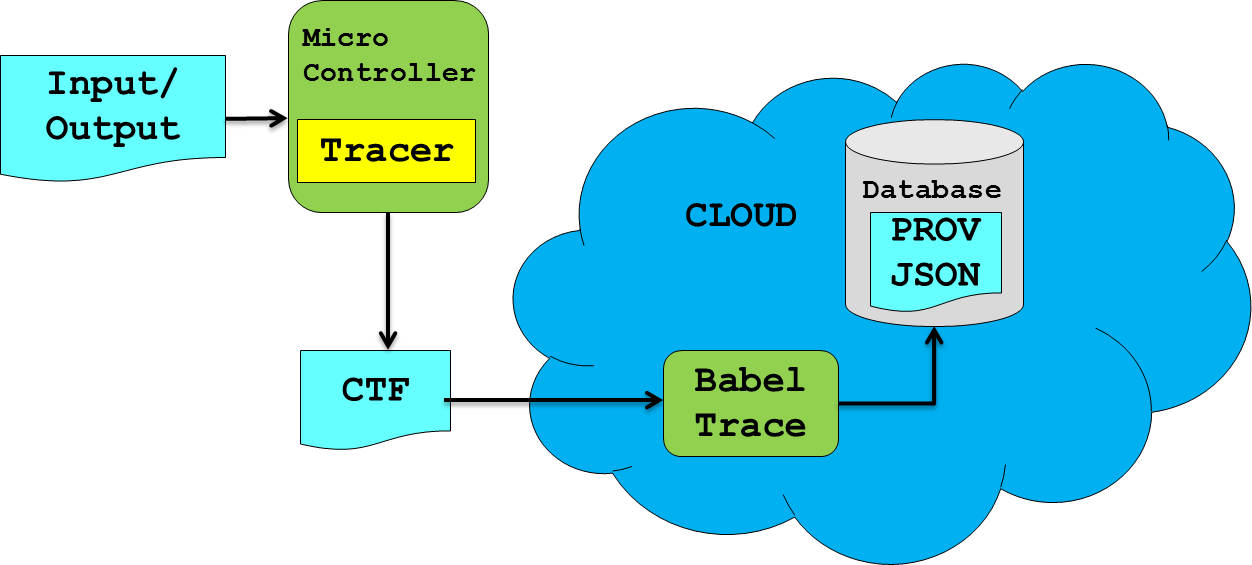
\includegraphics[width =3.0in]{system_architecture.PNG}    
\end{center}
\caption{System Architecture for Provenance Collection.}
\label{architecture}
\end{figure}

Our goal is to create a provenance-aware system which records I/O operations on data for devices connected in an IoT system. For our implementation, several tools and hardware components are utilized in the development of our prototype, outlined below:

\begin{itemize}
\item Raspberry Pi the microcontroller used to evaluate our approach. We choose Raspberry Pi because it is a representation of what can be found on an IoT gateway device and it has the capability to include custom hardware in programmable logic. Also, Raspberry Pi is a low cost, simple IoT demonstrator that was chosen for its high performance, on­board emulation, and IoT gateway projects can be programmed without additional need for hardware tools.

%\item Real Time Executive for Multiprocessor Systems (RTEMS) is an open source real­time operating system (RTOS) for embedded systems. This operating system is a typical RTOS that may be deployed in IoT devices.

\item Neo4j, a graph database which allows optimized querying of graph data. Since provenance represents causal dependencies, it is ideal to use a graph database to store the relationships between objects

%\item lttng, a software tool for collecting system level trace on Linux system. 

\item Babeltrace:  This is a trace converter tool. It contains plugins used to convert traces from one format into another. 

\item barectf: This is an application that collects bare metal application trace in CTF.

\item yaml generator: yaml generator creates yaml files. A yaml configuration file contains information on what barectf application needs in order to generate CTF trace output. This consist of configuration settings such as an application trace stream, packet type, payload type and size. 

%\item rasberrypi

\end{itemize}


\section{Application Use Case Implementation} \label{use_case_application}

To demonstrate the effectiveness of our framework, we implement an application of the smart home use case demonstrated in chapter 1 which serves as a prototype for proof of concept. In order to collect sensor-actuator trace data, I plan to create a sample application implemented on a microcontroller. I chose an application that simulates a smart home lock authentication system. This system uses facial recognition to recognize and grant access to a door lock. I plan to implement this using a web camera attached to the microcontroller. On the microcontroller is contained OpenCV, an open source software library developed for image processing. OpenCV allows for facial recognition on the microcontroller. Trace data generated from the smart home lock system in the form of CTF is collected on the microcontroller using barectf. CTF trace is translated to PROV-JSON which is stored in Neo4j, a graph database. Neo4j allows for querying and visualization of provenance. 




\section{Experiment Evaluation}

I plan to evaluate the effectiveness of my approach for provenance collection by using an intrusion detection system specifically developed for IoT. An IDS is used to detect malicious attacks using either a rule-based or an anomaly-based approach. A rule-based approach allows for intrusion monitoring by looking for specific known signatures of malicious attacks. An example of a signature-based IDS is an anti-virus software. An anomaly-based IDS identifies an intrusion by checking for patterns that falls out of the normal system behavior. Most anomaly-based approaches make use of machine learning to classify normal or anomalous behavior. These approaches can be useful to detect previously unknown malicious attacks. 
\par We propose a provenance-based IDS for IoT that extends Provenance-aware Intrusion Detection and Analysis System (PIDAS) \cite{Xie:2016:UID:2936026.2936232}, which uses system-level provenance data to provide real-time vulnerability intrusion detection on system behaviors. This system collects provenance from system calls. PIDAS contains three essential components: collector,detector and analyzer. The collector records provenance information of applications running in the user space. Provenance data is stored in a key-value pair database for easy query of acyclic graphs. The detector extracts dependency relationships from the provenance data and stores these relationships in a repository (BerkleyDB) for further analysis. The analyzer is responsible for identifies possible intrusion activities by making queries to view all dependencies from the suspected intrusion point. Provenance detector is made possible by using a provenance-based algorithm that matches the path contained in the graph.


The detector consists of three steps. Rule-built collects normal system behavior of provenance data and stores this information in a ruleDB. A ruleDB consists of a key-value pair which has parent and child relationships in the dependency graph. The rule-built is used to match observed provenance events  to detect system intrusion. Provenance information in the form of a dependency relationship is matched with the child-parent dependency rule information contained in the ruleDB. This information is used to compute the decision value which determines if there has been an intrusion. A description of the PIDAS rule matching and scoring algorithm is described in detail below: 

\begin{itemize}

\item provenance data is divided into dependency relationships, $Dep_1,...,Dep_n. Dep_i =(A, B)$. Where A is the parent of B

\item The scoring algorithm checks if there exists a match in the path between edges contained in the provenance dependency database, ruleDB. If there exists a path, a score of 1 is given to the path. This score is known as the path dubiety. Otherwise, if the path does not match any edge in the ruleDB, a score of 0 is given to the path.

Let R = provenance information of a program and G = provenance information contained in ruleDB. For each $Dep_i = (A, B) \in R, if Dep_i = (A, B) \in G$. Path dubiety = 1 else set intrusion dubiety = 0

\item The path decision, P is the sum of the dubiety of all the edges contained in the provenance graph divided by the number of edges in the provenance dependency database.

 \[P =\frac{\sum\limits_{i=1}^W dubeity of Dep_i }{W} \] P is compared with a threshold value, T. If P $>$ T, an anomaly exists in the system.

\end{itemize}

I plan to compare our proposed framework using PIDAS with a baseline which consists of an implementation of PIDAS on an embedded system. More specifically, I plan to evaluate the false negative and true positive rate for the IDS system as compared with the baseline. False positive dictates the number of times in which an intrusion has been wrongly detected. This signifies that a path contained in an applications provenance was detected and not found in the ruleDB. True positive rate identifies the number of times a intrusion has been detected. I also plan to evaluate the throughput of the system by evaluating the overhead incurred using the system.



%\section{Provenance Aware IDS System for IoT }
%
%This section outlines the core functionalities of our model PAIST. 
